

The dimension-free ``oracle" lower bounds that have been discussed up until this point rely upon a well-behaved objective function $f$ and constraint set $\mathcal{X}$ in the $\ell_2$ norm; namely, the radius of the constraint set $R$ and smoothness of the objective function with respect to the $\ell_2$ norm must be independent of the ambient dimension $n$ in order to achieve a dimension-free oracle bound. In some settings, $f$ and the support $\mathcal{X}$ may be well-behaved with respect to an arbitrary norm $\|\cdot \|$, in which we wish to exploit the underlying structure to achieve fast convergence rates. One possible example is minimizing the function $f$ over an $\ell_1$ ball. In this section, we provide an overview of the details of mirror descent, a method developed by \citet{blair1985problem}, which allows us to achieve a faster convergence rate for vector spaces endowed with an arbitrary norm. In this section, we follow the exposition of \citet{DBLP:journals/ftml/Bubeck15}.

\subsection{Background}
In order to extend our optimization methods to apply to arbitrary norms, we turn our focus to optimization procedures that work over any Banach space. Projected gradient descent does not apply to normed vector spaces which are not derived from an inner product since the gradients (which are linear functionals defined on the support $\mathcal{X}$) are elements of the dual space, so the gradient descent update $x - \eta \nabla f(x)$ cannot be used\footnote{That is adding $x \in \mathcal{X}$ and $\nabla f(x) \in \mathcal{X}^{*}$ -- its dual -- is not well-defined}. Note that in the Hilbert space case, the Hilbert space and its dual are isometric due to the Riesz representation theorem, so we can perform gradient descent $x - \eta \nabla f(x)$.

In order to exploit the underlying geometry of our function, we replace the Euclidean geometry of projected gradient descent with a more pertinent geometry for our problem. Instead of making the gradient update directly, mirror descent maps the point to the dual space and performs the gradient update before mapping it back to the primal space. This can be done due to the duality properties of the Bregman divergence.

For our arbitrary norm $\|\cdot \|$ on $\mathbb{R}^n$, we wish to minimize $\mathcal{X} \subset \mathbb{R}^n$. Our dual space is endowed with the dual norm $\|g \|_* = \sup_{\|x\|\leq 1} g^Tx$.

In mirror descent, the gradient of the mirror map $\Phi: \mathcal{D} \rightarrow \mathbb{R}$ is used to map points in the primal space to the dual space, the latter of which is where the gradient update takes place. In order to use the mirror map in this manner, we impose some conditions on $\Phi$.
\begin{itemize}
\item $\Phi$ is strictly convex and differentiable
\item $\nabla \Phi(\mathcal{D}) = \mathbb{R}^n$
\item $\lim_{x \rightarrow \partial \mathcal{D}} \|\nabla \Phi(x)\| = \infty$
\end{itemize}
These conditions guarantee that the map is invertible as well as provide conditions for the existence and uniqueness of a projection which we will see in the next subsection.

A natural generalization of the squared Euclidean norm is the Bregman divergence as it satisfies many similar properties. The Bregman divergence associated with $\Phi$ can be formally written as
$$ D_{\Phi}(x,y) = \Phi(x) - \Phi(y) - \nabla \Phi(y)^T(x-y)$$
This can be interpreted as the distance between the function at $x$ and the first-order Taylor expansion around $y$ for a given potential function $\Phi$. It is worth noting that the Bregman divergence is guaranteed to be non-negative when $\Phi$ is convex.

The Bregman divergence includes many classical examples of distances such as Mahalanobis distances and the Kullback-Liebler divergence. Several other useful properties of the Bregman divergence include:
\begin{itemize}
    \item The Bregman projection onto a convex set $\mathcal{X} \subset \mathbb{R}^n$ given by $y' = \arg\min_{x \in \mathcal{X}} D_{\Phi}(x,y)$ is unique.
    \item The generalized Pythagorean theorem for all $x \in \mathcal{X}$ and $y \in \mathbb{R}^n$, we have
    $$D_{\Phi}(x,y) \geq D_{\Phi}(x,y') + D_{\Phi}(y',y)$$
    where $y'$ is the Bregman projection of $y$ onto $\mathcal{X}$.
    \item Duality:
    $$D_{\Phi}(x,y) = D_{\Phi^*}(\nabla \Phi(x), \nabla \Phi(y))$$
    where $\Phi^*$ is the convex conjugate of $\Phi$.
\end{itemize}


\subsection{Mirror Descent}
\begin{figure}
    \centering
    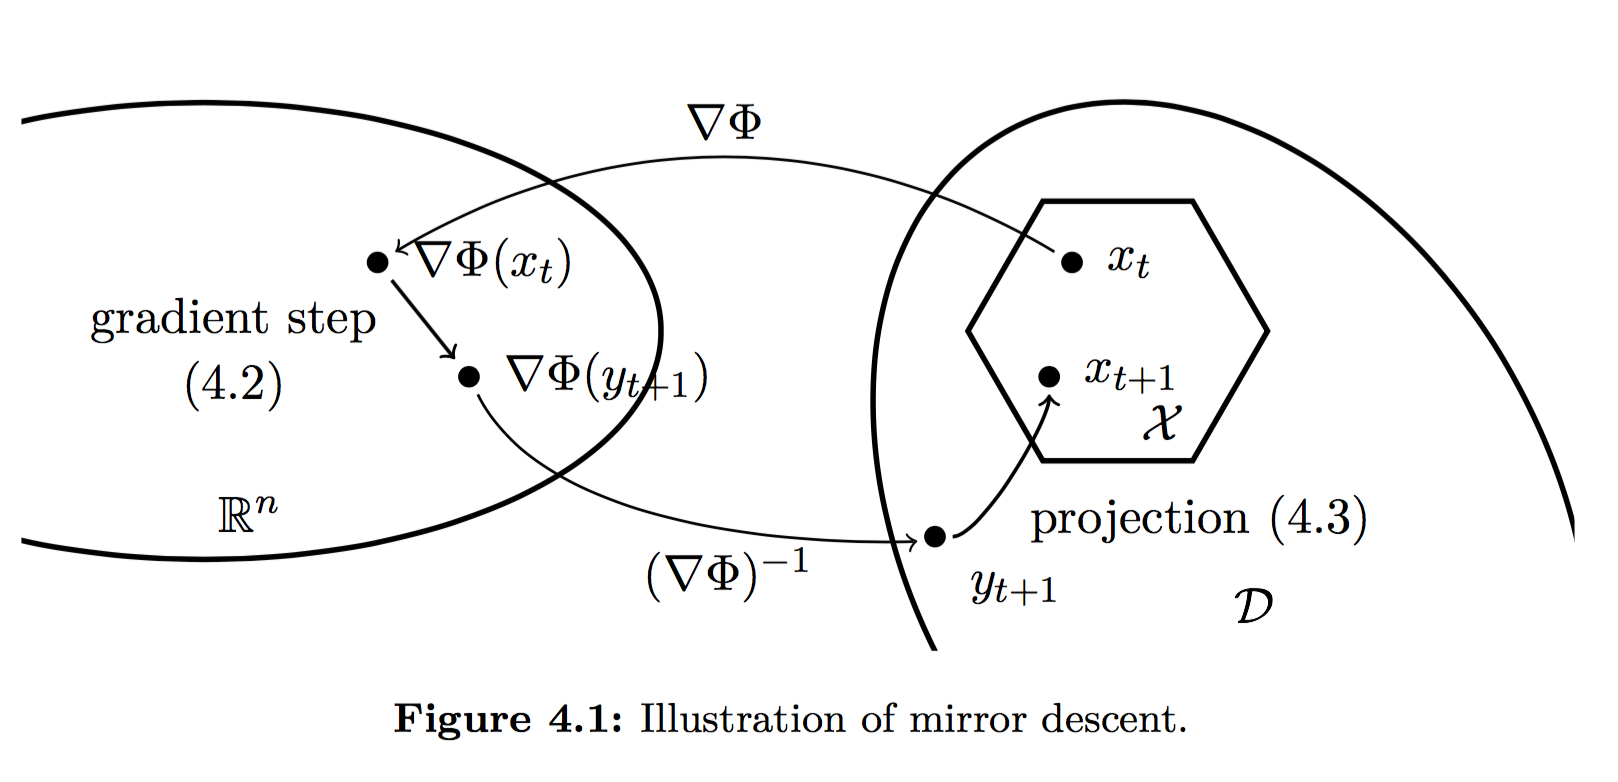
\includegraphics[width = 0.75\linewidth]{Images/mda.png}
    \caption{Illustration of Mirror Descent from \citep{DBLP:journals/ftml/Bubeck15}}
    \label{fig:my_label}
\end{figure}
The mirror descent algorithm can be described in two steps:
\begin{enumerate}
\item Perform the gradient update
\begin{align}
\label{md}
    \nabla \Phi(y_{t+1}) = \nabla \Phi(x_t) - \eta g_t
\end{align}
where $g_t \in \partial f(x_t)$
\item Project back onto $\mathcal{X}$
$$x_{t+1} \in \Pi_{\mathcal{X}}^{\Phi}(y_{t+1})$$
\end{enumerate}

We can rewrite the mirror descent algorithm from the proximal viewpoint
\begin{equation*}
x_{t+1} = \arg\min_{x \in \mathcal{X}\cap \mathcal{D}} \eta g_t^Tx + D_{\Phi}(x,x_t)
\end{equation*}
From this viewpoint, we choose a local linear approximation of $x_t$ in the direction of the subgradient while penalizing points far away from the previous point measured in terms of the Bregman divergence of the mirror map. Now with the algorithm in hand, we can proceed with the convergence results of the mirror descent algorithm.

\begin{theorem}
Let $\Phi$ be a mirror map $\rho$-strongly convex on $\mathcal{X} \cap \mathcal{D}$ with respect to $\|\cdot\|$. Let $R^2 = \sup_{x \in \mathcal{X}\cap \mathcal{D}} \Phi(x) - \Phi(x_1)$, and $f$ be convex, $L$-Lipschitz with respect to $\|\cdot\|$. Then mirror descent with $\eta = \frac{R}{L}\sqrt{\frac{2\rho}{t}}$ satisfies
\begin{equation}
f\Big(\frac{1}{t}\sum_{s=1}^t x_s\Big) - f(x^*) \leq RL\sqrt{\frac{2}{\rho t}}
\end{equation}
\end{theorem}
\proofstart The above bound will be obtained by taking the limit as $x \in \mathcal{X} \cap \mathcal{D}$ approaches $x^*$. Using convexity and the generalized Pythagorean theorem for Bregman divergences, we have
\begin{align*}
    f(x_s)-f(x) &\leq g_x^T(x_s - x) \\
    &= \frac{1}{\eta} (\nabla \Phi(x_s) - \nabla \Phi(y_{s+1}))^T(x_s - x) \\
    &= \frac{1}{\eta}\Big(D_{\Phi}(x,x_s) + D_{\Phi}(x_s,y_{s+1}) - D_{\Phi}(x,y_{s+1})\Big)\\
    &\leq \frac{1}{\eta}\Big(D_{\Phi}(x,x_s) + D_{\Phi}(x_s,y_{s+1}) - D_{\Phi}(x,x_{s+1}) - D_{\Phi}(x_{s+1},y_{s+1}) \Big)\\
\end{align*}
The first and third terms will result in a telescoping series when summing over $x_s$, so we seek to bound the other two terms. This can be done by exploiting the $\rho$-strong convexity of the mirror map and utilizing the algebraic property that $az - bz^2 \leq a^2/4b$ for all $z \in \mathbb{R}$. Bounding the second and fourth term,
\begin{align*}
    D_{\Phi}(x_s,y_{s+1}) - D_{\Phi}(x_{s+1},y_{s+1}) &= \Phi(x_s) - \Phi(x_{s+1}) - \nabla \Phi(y_{s+1})^T(x_s - x_{s+1}) \\
    &\leq (\Phi(x_s) -\nabla \Phi(y_{s+1}))^T(x_s - x_{s+1}) - \frac{\rho}{2}\|x_s - x_{s+1}\|^2\\
    &= \eta g_s^T(x_s - x_{s+1}) - \frac{\rho}{2}\|x_s - x_{s+1}\|^2\\
    &\leq \eta L \|x_s - x_{s+1}\| - \frac{\rho}{2}\|x_s - x_{s+1}\|^2\\
    &\leq \frac{(\eta L)^2}{2\rho}
\end{align*}
Thus,
$$\sum_{s=1}^t \Big(f(x_s) - f(x)\Big) \leq \frac{D_{\Phi}(x,x_{1})}{\eta} + \eta \frac{L^2 t}{2\rho}$$
which can be rewritten as the theorem statement \proofend 

This rate verifies the properties of mirror descent, which we expanded upon earlier in the section.

To gain intuition for settings in which mirror descent proves useful, we expand upon some standard setups in which mirror descent is commonly used.
\begin{itemize}
\item $\ell_2$-ball - Choosing the mirror map as the squared Euclidean norm on $\mathcal{D} = \mathbb{R}^n$
$$\Phi(x) = \frac{1}{2}\|x\|_2^2$$
induces a Bregman divergence of $D_{\Phi}(x) = \frac{1}{2}\|x - y\|_2^2$ which coincides with standard projected subgradient descent.
\item $\ell_1$-ball - Another commonly used mirror map is negative entropy
$$\Phi(x) = \sum_{i=1}^n x(i) \log x(i)$$
where $\mathcal{D} = \mathbb{R}^n_{++}$. The associated Bregman divergence is the KL-divergence $D_{\Phi}(x,y) = \sum_{i=1}^n x(i) \log \frac{x(i)}{y(i)}$. Projecting onto the simplex can be achieved by simply re-normalizing $y \rightarrow y/\|y\|_1$. In this case, when the subgradients of $f$ are bounded in the $\ell_{\infty}$-norm, the convergence rate of mirror descent is $\sqrt{\frac{\log n}{t}}$ while the convergence rate of subgradient descent is $\sqrt{\frac{n}{t}}$.
\end{itemize}

It is worth noting to conclude that although any convergence rate on the $\ell_1$ norm can be bounded in terms of the $\ell_2$ norm, this may introduce the ambient dimension $n$ preventing us from properly exploiting the geometry of the problem at hand.

\subsection{Dual Averaging}
A slightly more computationally efficient version of mirror descent is called Nesterov's dual averaging (which can also be exploited in distributed settings). Instead of mapping between the primal and dual space during each step, dual averaging averages the gradients in the dual space, so we replace $\nabla \Phi(y_{t+1}) = \nabla \Phi(x_t) - \eta g_t$ with
$$\nabla \Phi(y_{t+1}) = \nabla \Phi(y_t) - \eta g_t$$
then the update equation is
$$x_t = \arg\min_{x \in \mathcal{X} \cap \mathcal{D}} \eta \sum_{s=1}^{t-1}g_s^Tx + \Phi(x)$$
\begin{theorem}
Let $\Phi$ be a $\rho$ strongly convex mirror map on $\mathcal{X} \cap \mathcal{D}$ with respect to $\|\cdot \|$. Let $R^2 = \sup_{x \in \mathcal{X} \cap \mathcal{D}} \Phi(x) - \Phi(x_1)$, and $f$ be convex and $L$-Lipschitz wrt $\|\cdot\|$. The dual averaging mirror descent 
$$f\Big(\frac{1}{t}\sum_{s=1}^t x_s \Big) - f(x^*) \leq 2RL \sqrt{\frac{2}{\rho t}}$$
\end{theorem}
\proofstart Define the $\rho$-strongly convex update equation as $\psi_t(x) = \eta\sum_{s=1}^{t-1}g_s^Tx + \Phi(x)$. Then from the first order optimality condition
$$\psi_t(x_{t+1}) - \psi_t(x_t) \leq -\frac{\rho}{2}\|x_{t+1} - x_t\|^2$$
In addition, we have
$$\psi_t(x_{t+1}) - \psi_t(x_t) \geq \eta g_t^T(x_{t+1} - x_t)$$
Combining the above two and using Cauchy-Schwarz yields
$$\frac{\rho}{2}\|x_{t+1} - x_t\|^2 \leq \eta g_t^T(x_{t} - x_{t+1}) \leq \eta L \|x_{t} - x_{t+1}\|$$
$$g_t^T(x_{t} - x_{t+1}) \leq \frac{2\eta L^2}{\rho}$$
Now it remains to be shown that combining with the above yields the desired bound 
$$\sum_{s=1}^{t}g_s^T(x_s - x) \leq \sum_{s=1}^{t}g_s^T(x_{s} - x_{s+1}) + \frac{\Phi(x) - \Phi(x_1)}{\eta}$$
This can be rewritten as
$$\sum_{s=1}^{t}g_s^Tx_{s+1} + \frac{\Phi(x_1)}{\eta} \leq \sum_{s=1}^tg_s^Tx + \frac{\Phi(x)}{\eta}$$
which we can prove by induction. 
\proofend

